\chapter[Single-Crystal EPR on FeFe-Hydrogenase Hox state]{Single Crystal EPR on the H$_{ox}$ state of FeFe-Hydrogenase\blfootnote{Portions of this text are from J.~W.~Sidabras, J.~Duan, M.~Winkler, T.~Happe, R.~Hussein, A.~Zouni, D.~Suter, A.~Schnegg, W.~Lubitz, E.~J.~Reijerse, Sci. Adv., {\em accepted}.}}

Nature has evolved enzymes with various metallic cofactors (metallo-enzymes) to efficiently catalyze energy conversion reactions. These enzymes, which include, for example, photosystem II oxygen evolving complex\cite{CoxOEC}, hydrogenases\cite{lubitzhyd}, nitrogenases\cite{Hoffman2014rev}, and CO dehydrogenase\cite{C5CS00182J}, employ first-row transition metals to perform their catalytic functions. One of the main challenges is to fully understand these enzymatic mechanisms and provide a basis for cheap, robust, and highly active molecular catalysts designed for practical applications. \cite{Lewis15729} The ultimate goal is to alleviate the requirement of noble metals, such as platinum, that limit the scalability of current technology. This important biophysical and biochemical research seeks metallo-enzyme based and inspired systems as an interesting route to advance towards the future of clean energy and efficient energy storage. \cite{schlogl2012chemical}

The catalytic cycle of redox enzymes often contain paramagnetic intermediates and EPR is the method of choice used to study these occurrences. Through EPR experiments, information on the magnetic and geometrical structure of the active site can be obtained. EPR spectroscopy can probe isolated intermediates in the catalytic cycle when either a single unpaired electron or multiple unpaired electrons with magnetic couplings are present in the ground state. Fundamentally understanding such enzymes is of broad biochemical and biophysical importance as we move towards bioengineering mimics of nature’s most elusive chemistry. \cite{WATANABE20171}

One such interesting class of metallo-enzymes are the hydrogenases\cite{lubitzhyd} which catalyze the conversion of molecular hydrogen H$_2$, such that,
\begin{equation}
    \text{H}_2 \rightleftharpoons 2 \text{H}^+ + 2\text{e}^{\text{-}}.
\end{equation}
Hydrogenases are key enzymes in many organisms for hydrogen metabolism regulation in the cell or are used as electron donors for processes further down energy conversion pathways. The hydrogenase enzyme family has three distinct active-sites with different mechanistic hydrogen conversion. These mechanisms utilize either a single-iron center [Fe], a bi-nuclear iron [FeFe], or a nickle-iron [NiFe] active-site for catalysis.

Of great interest is the bi-nuclear [FeFe]-hydrogenase. \cite{PETERS20151350} These enzymes are amongst the fastest on the planet (turn-over frequencies over 10,000 s$^{\text{-1}}$ \cite{CatalyticTOF}) and provide a potential route to sustainable hydrogen production. The proposed crystal structure of one such hydrogenase from {\em Clostridium pasteurianum} (CpI) highlighting the active site and electron-transfer pathway is shown in Fig.~\ref{fig:CpIGeo}A. The electron-transfer pathway involving accessory iron-sulfur clusters is indicated as a solid blue arrow. In CpI, a [2Fe2S] cluster is found symmetric to the electron-transfer pathway, illustrated as a dashed blue line, and is believed to ``tune'' the redox potentials of the [4Fe4S] clusters. \cite{PetersPotentials} The [FeFe]-hydrogenase active-site carries a [4Fe4S] cluster linked via a cysteine ligand connecting the [2Fe]-cofactor molecule. The [2Fe]-cofactor contains an iron atom proximal (Fe$_p$) and one distal (Fe$_d$) to the [4Fe-4S] cluster. Each iron carries a cyanide (CN$^-$) and one carbonmonoxide (CO) ligand and the two irons share a bridging carbonmonoxide ($\mu$CO). Additionally, the two iron atoms are bridged by an azapropane-dithiolate-ligand (ADT-ligand). The molecular structure of the [FeFe]-hydrogenase active site, known as the H-cluster, can be found in Fig.~\ref{fig:CpIGeo}B. The whole active site has a total of six iron atoms at various redox states in the catalytic cycle. In the vicinity of the H-cluster, there exists proton (2H$^+$; illustrated as a dashed red line) and molecular hydrogen (H$_2$; illustrated as a solid red line) channels for gas exchange. Through many spectroscopic techniques, such as, Fourier Transform Infra-Red (FTIR), EPR, Nuclear Magnetic Resonance (NMR), M\"o\ss{}bauer, Raman, and Nuclear resonance vibrational (NRVS), a convincing catalytic cycle has been hypothesized. \cite{lubitzhyd, NRVS2017, sommer2017} However, more work must be done to fully understand the catalytic mechanism and relate it to quantum chemical calculations. 

\begin{figure}[htpb]
\centering
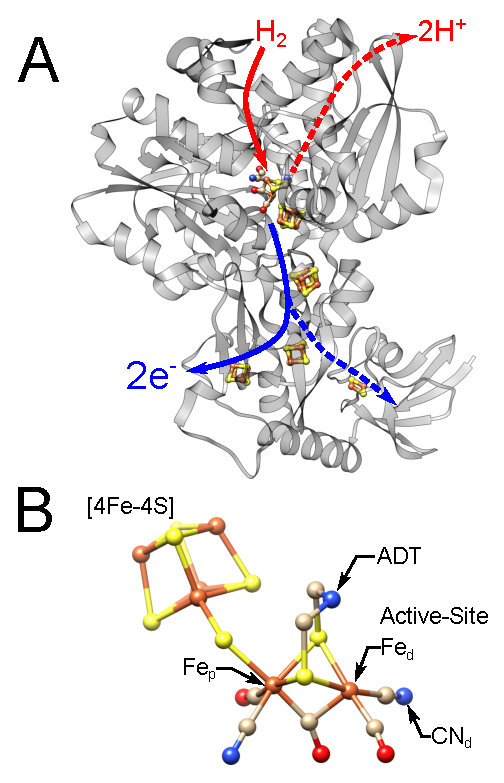
\includegraphics{Kapitel/Ch1-images/CpI-geometry.eps}
\caption[Crystal structure of {\em Clostridium pasteurianum} (CpI).]{A) Crystal structure of {\em Clostridium pasteurianum} (CpI) from PDB ID 4XDC. The [Fe-Fe]-Hydrogenase CpI is a 64~kDa protein with four [4Fe4S] clusters and one [2Fe2S] cluster. The iron-sulfur  clusters  are involved  in  the electron\-/transfer  pathway (solid blue). A [2Fe2S] cluster is found symmetric to the [4Fe4S] pathway (dashed blue) and is believed to ``tune'' the redox potentials of the nearby [4Fe4S] clusters. There exists a proton (2H$^+$;dashed red) and hydrogen (H$_2$; solid red) channel for gas exchange. The active-site, or H-cluster, resides at the top in this view and is B) expanded to show the H-cluster structure. Within the H-cluster, the proximal iron (Fe$_p$) and distal iron (Fe$_d$) of the [FeFe]-hydrogenase is shown. In this view, Fe is orange, S is yellow, N is blue, O is red, and C is beige.}
 \label{fig:CpIGeo}
\end{figure}

Using frozen solution samples, EPR spectroscopy has been used to study the paramagnetic states of [FeFe]-hydrogenase from a number of organisms. \cite{lubitzhyd,Silakov57Fe,Adamska2015pdt,Adamska2015} These experiments have determined the magnetic principal \textit{g}-values, hyperfine, and quadrupole parameters for the catalytic states with EPR active co-factors and [4Fe4S] clusters. Such important intermediate states include H$_{ox}$ and H$_{sred}$ in the catalytic cycle, a reversible carbon monoxide (CO) inhibited H$_{ox}$-CO state, and any state with reduced [4Fe4S] clusters, including the \textit{apo}-HydA protein which lacks the H-cluster. In this work we focus on H$_{ox}$ which is the primary catalytic state of the [FeFe]-hydrogenase.

It was found that an {\em Escherichia coli} ({\em E. coli}) expressed \textit{apo}-HydA could be combined with an artificially synthesized H-cluster to form fully functional [FeFe]\-/hydrogenase. \cite{EsselbornArtificial, BirrellArtificial} This has not only increased the yields of the precursor of the binuclear co-factor but has allowed synthetically modified co-factors to be inserted and a wealth of information has been obtained, including the identification of the head group in the bridging ADT-ligand. \cite{AdamskaBridgingAmine} With this tool, it became possible to enrich the H-cluster with magnetic isotopes and study the corresponding magnetic interactions. These experiments allowed the synthesis of $^{57}$Fe in the binuclear  co-factor, $^{13}$C, $^{14}$N, and $^{15}$N in the CN$^-$ and ADT ligands, and $^{13}$C in the CO ligands. A summary of the magnetic properties of the H$_{ox}$ state can be found in Table~\ref{table:eprthing}. 

\begin{table}[hb]
\caption[EPR parameters determined for FeFe-hydrogenase in Hox state.]{EPR parameters determined by frozen solution of [FeFe]-hydrogenase in the H$_{ox}$ state through a series of pulse EPR experiments.}
\centering
\begin{tabular}{l|c|c||c}
 & Fe$_p$ $^\dagger$ & Fe$_d$ $^\dagger$ & {[}4Fe4S{]} \\ \hline \hline
oxidation state & II & I & 2+ \\
Spin state & $S=0$ & $S=1/2$ & $S_{eff}=0$ \\
$g$-values & -- & {[}2.100, 2.040, 1.999{]} & -- \\
A (MHz) & {[}12.3, 11.4, 12.6{]} & {[}12.3, 11.4, 12.6{]} & $\pm${[}11.2, 10.4, 11.6{]} \\
{[}$\alpha$, $\beta$, $\gamma${]} (deg) & {[}0, 0, 0{]} $\pm$30 & {[}0, 0, 0{]} $\pm$30 & {[}0, 0, 0{]} $\pm$30
\end{tabular}
\begin{flushleft}\footnotesize{$^\dagger$ From DFT calculations of Ref.~[1.\kern-0.4em\citenum{GrecoDFT}], we assume the majority of the spin is located on Fe$_d$; however, significant $^{57}$Fe hyperfine interactions on both irons are measured by Silakov {\em et al.} in Ref.~[1.\kern-0.4em\citenum{Silakov57Fe}].} \end{flushleft}

\begin{tabular}{l|c|c|c}
& C$^{15}$N$_d$ $^\ddagger$ & C$^{14}$N$_d$ $^\ddagger$ & ADT-Ligand ($^{14}$N)$^{\ddagger^\ddagger}$\\ \hline \hline
A (MHz) &  {[}-1.3, -1.1, 6.2{]} & {[}-0.9, -0.8, 4.4{]} & {[}1.35, 1.15, 1.15{]}\\
{[}$\alpha$, $\beta$, $\gamma${]} (deg) & {[}-90, -50, 0{]}$^\ast$ & {[}-90, -50, 0{]}$^\ast$ & {[}0, 0, 0{]}\\
$P_{||}$ {[}MHz{]} &  -- & 0.9 & 1.23\\ 
$\eta$ & -- & 0.34 & 0.13 \\
{[}$\alpha$, $\beta$, $\gamma${]} (deg) & -- & {[}-46, -119, 0{]}$^\ast$ & {[}0, -90, 0{]}$^\ast$
\end{tabular}
\begin{flushleft}\footnotesize{$^\ddagger$ Data is obtained from Adamska {\em et al.} of Ref.~[1.\kern-0.4em\citenum{Adamska2015}]. Other groups, such as Britt and colleagues in Ref.~[1.\kern-0.4em\citenum{BrittLigands2014}] have obtained similar values; however, Adamska {\em et al.} use the same molecular frame described in this work. 

$^{\ddagger^\ddagger}$ Data is obtained from Adamska {\em et al.} of Ref.~[1.\kern-0.4em\citenum{Adamska2015pdt}]. 

$^\ast$ The Euler angles are in the new EasySpin Euler definition (since version 5.0), which required the transformation $[\alpha,\beta,\gamma]= -[\gamma,\beta,\alpha]$ from the published results.} \end{flushleft}

\begin{tabular}{l|c|c}
 & $^{13}$CN$_p$ $^\ddagger$ & $^{13}$CN$_d$ $^\ddagger$  \\ \hline \hline
A (MHz) & {[}5.52, 5.52, 4.55{]} & {[}30, 28.5, 22.7{]} \\
{[}$\alpha$, $\beta$, $\gamma${]} (deg) & {[}0, 0, 0{]}  \\
\end{tabular}
\begin{tabular}{l|c|c|c}
 & $^{13}$CO$_p$$^{\ast\ast}$ & $^{13}$CO$_d$$^{\ast\ast}$ & $\mu^{13}$CO$^{\ast\ast}$ \\ \hline \hline
A (MHz) & {[}5.52, 5.52, 4.55{]} &  {[}20.5, 29.9, 26.0{]} & {[}9.0, 3.8, 4.5{]}\\
{[}$\alpha$, $\beta$, $\gamma${]} (deg) &  {[}25, 25, 0{]} & {[}37, 26, 0{]} & {[}0, 20, 0{]} \\
\end{tabular}\label{table:eprthing}

\begin{flushleft}\footnotesize{$^{\ast\ast}$ Data is obtained from Britt {\em et al.} of Ref.~[1.\kern-0.4em\citenum{BrittC13}].} \end{flushleft}
\end{table}

The data in Table~\ref{table:eprthing} represents the current knowledge on the magnetic properties of the [FeFe]-hydrogenase in the H$_{ox}$ state. However, this table is not exhaustive and further information on both the magnitude and orientation of the \textit{g}-, hyperfine-, and quadrupole-tensors is still needed. To date, quantum chemical calculations have difficulties in predicting the principal values of the \textit{g}-tensor\cite{GrecoDFT, FiedlerDFT} and are only used to qualitatively assign spin densities when simulating interactions with surrounding nuclei. From the current literature, it is not clear on what amino acids are involved in the first ligand-sphere and, therefore, single crystal EPR experiments are needed to properly determine the full-magnetic interactions of the H-cluster. 

In this work, advancement to the state-of-the-art EPR instrumentation is achieved in order to improve both frozen solution data acquisition methods and obtain the ability to measure protein single crystals with dimensions less than 0.3~mm$^3$. From the EPR single crystal data, past studies using assumptions and speculations of the \textit{g}-tensor and how it relates to the surrounding nuclei can be refined or abandoned; while, quantum chemical calculations of the magnitudes and orientations of the magnetic tensors can be tested by comparing to experimental data.

Using the photosystem II Y$_D^\bullet$ radical in Chapter~5, we have established that the self-resonant micro-helix is suitable for studies of single-crystal protein samples of volumes less than 27~nL. The self-resonant micro-helix is optimal for these experiments due to the relatively large bandwidth (90~MHz critically-coupled), efficiency of 3.2~mT/W$^{1/2}$, which corresponds to a $\pi/2$ pulse of as short as 20~ns with an incident power of only 20~mW, and the relatively homogeneous microwave magnetic field incident on the sample. We now want to demonstrate that i) a full angular $g$-tensor determination can be performed and, due to the six fold signal enhancement, that ii) advanced pulse EPR experiments, like ESEEM and HYSCORE, in single crystals are not only feasible, but useful. 

We report here, for the first time, a proposed $g$-value from field-stepped ESE rotational data and HYSCORE derived data for a [FeFe]-hydrogenase in the active oxidized state (H$_{ox}$) from {\em Clostridium pasteurianum} in a 0.3 $\times$ 0.1 $\times$ 0.1~mm$^3$ crystal volume. These data demonstrate the utility of the micro-helix in studying protein single-crystals at sizes relevant for X-ray crystallography.

\section{Methods}
The [FeFe]-hydrogenase from {\em Clostridium pasteurianum} (CpI) was grown and crystallized to a size of 0.3 $\times$ 0.1 $\times$ 0.1~mm$^3$ by the method of Esselborn {\em et al.}\cite{FeFeCry} under auto-oxidative conditions, i.e. without reducing agents. This leaves the enzyme in the characteristic active oxidized state (H$_{ox}$), giving rise to a $S=1/2$ ground state of the H-cluster. The accessory iron-sulfur clusters in the protein are oxidized and remain EPR silent. \cite{lubitzhyd}  Under a microscope in an anaerobic chamber, the protein crystal is drawn by capillary action into a 0.3~mm inner diameter capillary with mother liquor and cryoprotectant, centered in the micro-helix, and flash frozen. The micro-helix assembly is affixed to the EPR probehead, placed in a pre-cooled cryostat, and attached to the EPR bridge. The whole micro-helix probehead is then rotated in 5$^{\circ}$ steps over 180$^{\circ}$ in one-plane within the magnet. 

\begin{figure}[htbp]
\centering
 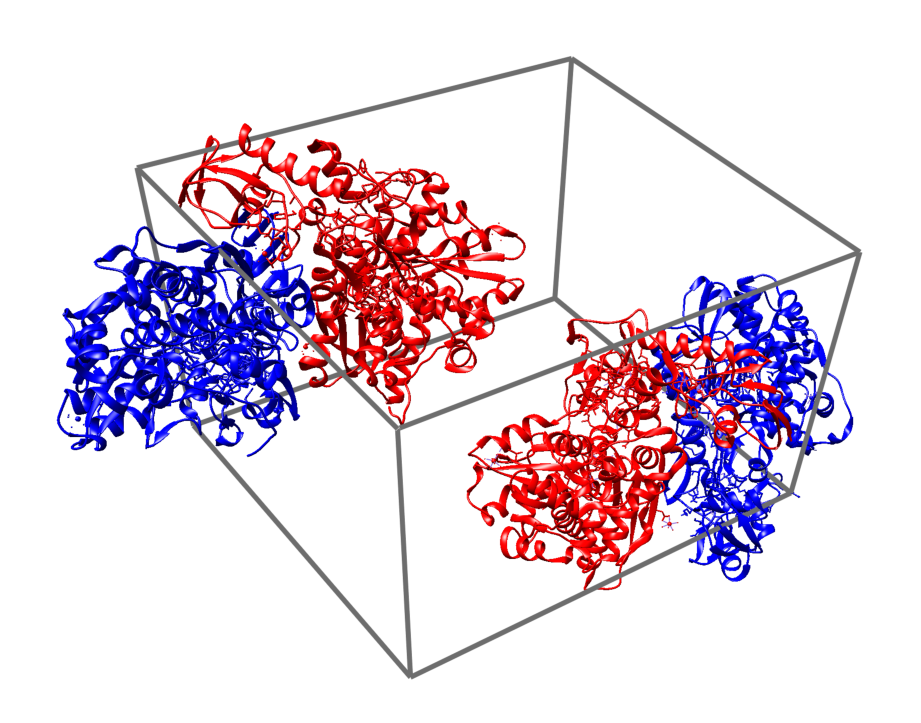
\includegraphics[width=0.5\textwidth]{Kapitel/Ch6-Images/Ch6-UnitCell.eps}
 \caption[Unit Cell from PDB 4XDC.]{Shown is the unit cell of PDB ID 4XDC with the molecules in an asymmetric unit (red and blue) and copied by the P$1\,2_1\,1$ symmetry.} 
 \label{fig:xTalFeFeUnit}
\end{figure}

The [FeFe]-hydrogenase of {\em Clostridium pasteurianum} (CpI) has a molecular weight of 67~kDa. The unit cell has P$1\,2_1\,1$ symmetry with two molecules in the asymmetric unit (PDB ID: 4XDC), shown in Fig.~\ref{fig:xTalFeFeUnit}. Each of the four enzymes per unit cell contain one active-site (H-cluster, shown in Fig.~1.1B in Chapter~1) which results in four distinct signals. The single crystal had a volume of approximately 0.3 $\times$ 0.1 $\times$ 0.1~mm$^3$ and, based on the unit cell dimensions, approximately 17$\times10^{12}$ enzymes within the crystal are calculated. The four observed signals corresponding to 4.25$\times10^{12}$ spins per peak. 

In the current setup, the entire probe head is rotated within the magnet with the static magnetic field in the laboratory frame $L_1$-direction and rotation takes place on axis of the microwave magnetic field in the $L_3$-direction, per Fig.~2.6A in Chapter 2. Since the setup is axially symmetric, this allows for full rotation in one crystal plane over 180 degrees. The laboratory frame is set in the EasySpin simulations and the collected spectra are fitted using the Matlab programs supplied in Appendix~3 or at: https://act-epr.org/data. The \textit{esfit} routine was modified with a sub-routine employing partial parallelization of the simulations. This allowed for 12 spectra in 3 chunks to be simulated simultaneously for a total of 36 spectra per fit. A particle swarm optimization algorithm with 10,000 particles (fits) was used to find the solution. Each run was allowed to converge in 10 iterations and checked if a local minimum was found. The Easyspin solution took about 1~second for each fit for a total of approximately 2.5~hours per iteration. Simulations were re-run until a good fit was established.

The simulation is setup with 9 unknowns: the three axes of the crystal frame that relates how the crystal is orientated in the laboratory frame, the three axes of the g-tensor of the first molecule (g-Tensor A) and how it relates to the Molecular-Frame A, and the three axes of the g-tensor of the second molecule (g-Tensor B) and how it relates to the Molecular-Frame B. However, we can assume that the g-tensor of the second molecule will be almost the same as the first molecule, based on similar research at W-band with photosystem II. \cite{Hofbauer6623, B908093G} From this knowledge, we can limit the deviation of the $g$-tensor of the second molecule ($g$-tensor B) with respect to the first ($g$-tensor A). The crystal frame and $g$-tensor A were set to vary from a whole rotation. We assume that $g$-tensor B has minimal deviation from the solution of $g$-tensor A. Therefore we limited the $g$-tensor variation to only 15 degrees different compared to $g$-tensor A. The principal $g$-values were obtained from previous frozen solution EPR experiment in Ref.~[6.\kern-0.4em\citenum{lubitzhyd}] ($g$-values: [1.999, 2.039, 2.097] corresponding to $x$, $y$, and $z$, respectively).

The HYSCORE experiment has a ${\pi/2\!-\!\tau\!-\!\pi/2\!-\!t_1\!-\!\pi\!-\!t_2\!-\!\pi/2}$ pulse sequence which results in an echo $\tau$ seconds after the last $\pi/2$ pulse. The values for $t_1$ and $t_2$ are swept to form a 2D experiment at a fixed magnetic field position. Herein, the magnetic field is set to one of the peaks measured in the two-pulse ESE experiment, $\tau$ is 280~ns, $t_1$ and $t_2$ start at 300~ns with 256 48~ns steps, and $\pi$-pulse is 80~ns at a microwave power of 7~mW. 

\section{Results and Discussion}
\subsection{Pulse EPR in Single Crystals of [FeFe]-Hydrogenase.}
\begin{figure}[htbp]
\centering
 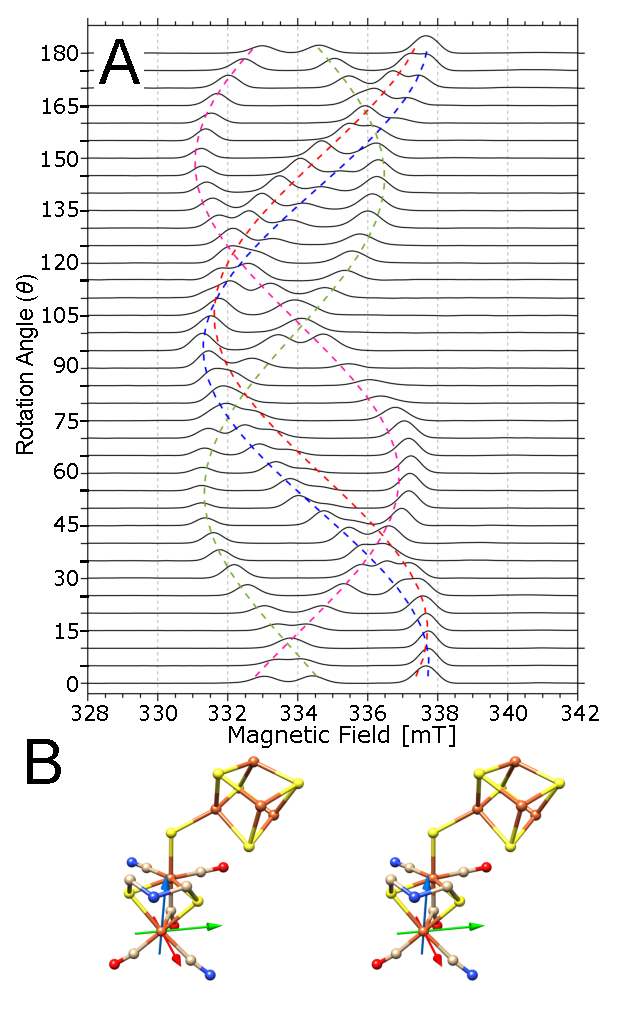
\includegraphics{Kapitel/Ch5-Images/04-FeFe-xTal-DataBig.eps}
 \caption[Pulse EPR on single-crystal of the H-cluster in FeFe-hydrogenase.]{A) Pulse EPR on single-crystal [FeFe]-hydrogenase of {\em Clostridium pasteurianum} (CpI) in the H$_{ox}$ state showing collected data in one plane for a full rotation of 180$^{\circ}$ in 5$^{\circ}$ steps at a temperature of 15~K. B) A stereo view of the analyzed $g$-tensor (g$_x$: green, g$_y$: blue, g$_z$: red) is mapped on the crystal structure (PDB ID: 4XDC). We assume that the order of the principal values of the $g$-tensor is $g_z\geq g_y\geq g_x$. For a 3D view of the proposed $g$-tensor see: https://act-epr.org/FeFeHydrogenase.html} 
 \label{fig:xTalFeFe}
\end{figure}

First, a field-swept two-pulse electron spin-echo EPR experiment was performed every 5$^{\circ}$ on a protein single-crystal of the [FeFe]-hydrogenase of {\em Clostridium pasteurianum} (CpI) in the oxidized H$_{ox}$ state and plotted in Fig.~\ref{fig:xTalFeFe}A. A very good signal-to-noise ratio of approximately 290 is calculated for a collection time of 8~minutes for each spectrum at a temperature of 15~K. 

From these spectra, the data can be fitted to simulations which relate the different frames of reference to each other as defined in the EasySpin simulation package. Rotational matrices for the relationship of these frames can be found in Table~\ref{table:frames}. The rotational matrices are found from the Euler angles found from the fitting of the laboratory and $g$-tensor frames. The resonance roadmap is overlaid on the field-swept two-pulse electron spin-echo EPR experiment shown in Fig.~\ref{fig:xTalFeFe}A. A second experiment with the same crystal was peformed and can be found in Appendix D Figs.~D.1 and D.2. The measurement in the second plane provides confidence in the fit of the $g$-tensor. A very good fit in both experiments was found. 

\begin{table}[ht]
\caption[Rotational matrices for the crystal frame.]{Rotational matrices  for the crystal frame with respect to the laboratory frame and the $g$-tensor with respect to the molecular frame. The crystal frame and $g$-tensor are found by fitting the data in Fig.~\ref{fig:xTalFeFe}A with the molecular frame from PDB ID 4XDC.}
\centering
\hspace{-12.825em}
\begin{tabular}{r|ccc}
 & \multicolumn{3}{c}{Crystal Frame} \\
\multicolumn{1}{l|}{} & $a$ & $b$ & $c$ \\ \hline \hline
L$_1$ & $+$0.273 & $-$0.162 & $-$0.948 \\
L$_2$ & $-$0.022 & $-$0.987 & $+$0.162 \\
L$_3$ & $-$0.962 & $+$0.023 & $-$0.273
\end{tabular}\label{table:frames} \\
\vspace{0.5cm}
\begin{tabular}{r|ccc|ccc}
 & \multicolumn{3}{c|}{Molecular-Frame A} & \multicolumn{3}{c}{Molecular-Frame B} \\
 & $x$ & $y$ & $z$ & $x$ & $y$ & $z$ \\ \hline \hline
$a$ & $-$0.331 & $-$0.938 & +0.107 & $-$0.595 & $-$0.666 & $-$0.450 \\
$b$ & $-$0.770 & +0.203 & $-$0.605 & +0.456 & $-$0.740 & +0.494 \\
$c$ & +0.545 & $-$0.283 & $-$0.789 & $-$0.662 & +0.089 & +0.744
\end{tabular}\\
\vspace{0.5cm}
\begin{tabular}{r|ccc|ccc}
 & \multicolumn{3}{c|}{\textit{g}-Tensor A} & \multicolumn{3}{c}{\textit{g}-Tensor B} \\
 & $x$ & $y$ & $z$ & $x$ & $y$ & $z$ \\ \hline \hline
$a$ & $+$0.476 & $-$0.484 & $+$0.735 & $+$0.377 & $-$0.605 & $-$0.701 \\
$b$ & $-$0.400 & $+$0.625 & $+$0.671 & $-$0.388 & $+$0.584 & $-$0.713 \\
$c$ & $+$0.783 & $+$0.613 & $-$0.103 & $+$0.841 & $+$0.541 & $-$0.015
\end{tabular}
\end{table}

The proposed $g$-tensor orientation is plotted as a stereo view in Fig.~\ref{fig:xTalFeFe}B. The $g$-tensor (g$_x$: green, g$_y$: blue, g$_z$: red) is presented with the origin at the distal iron (Fe$_d$), since Fe$_d$ is known to contain most of the spin density in the H$_{ox}$ state. \cite{FiedlerDFT,GrecoDFT} The $g$-tensor orientation found here is close to that proposed by Adamska {\em et al.} using HYSCORE measurements in frozen solution. \cite{Adamska2015} Direct comparison of the two proposed $g$-tensors can be found in Fig.~\ref{fig:gTensor}. 

Adamska {\em et al.} could simulate and calculate a hypothetical $g$-tensor that would give rise to the measured HYSCORE spectra. From this calculation, it was proposed that the g$_z$-axis lies along the Fe$_p$-Fe$_d$ axis in order to fit a CN$_d^-$-Fe$_d$-g$_z$ angle of 117$^\circ$ as shown in Fig.~\ref{fig:gTensor}A. The g$_x$-axis was chosen to point along the Fe$_d$ to ADT-amine nitrogen axis in order to bisect the nitrogen which is believed to be part of the formation of the hydride. The data collected using single-crystal EPR in this work is in good agreement with Adamska {\em et al.} and shows a deviation of only 10.1$^{\circ}$ from the axes previously proposed, shown in Fig.~\ref{fig:gTensor}B. However, the newly proposed $g$-tensor orientation has the $x$-axis pointing outward at the open coordination site and a 9.1$^{\circ}$ deviation from bisecting the H-cluster. These rotations cannot be found with frozen solution data and are only available with single-crystal experiments. No assumptions are made in the fitting of the $g$-tensor from single-crystal data. Further analysis and refinement is possible with the collection of hyperfine and quadrupole data originating from the same crystal and relating the whole dataset to quantum chemical calculations.

\begin{figure}[ht]
\centering
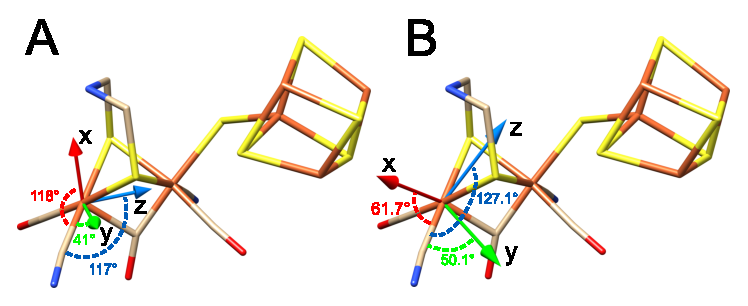
\includegraphics{Kapitel/Appendix/Images/S6-gTensorCompare.eps}
\caption[Comparison of the proposed $g$-tensor.]{A) The proposed $g$-tensor by Adamska {\em et al.} overlaid onto the H-cluster from PCB ID 3C8Y. (Adapted from Ref.~[6.\kern-0.4em\citenum{Adamska2015}] with permission from the PCCP Owner Societies.) B) The proposed $g$-tensor of this work overlaid onto the H-cluster from PCB ID 4XDC.}
\label{fig:gTensor}
\end{figure}

\subsection{Advanced Pulse EPR on the H-cluster in Single Crystals.}
Due to the excellent signal-to-noise of the field-stepped ESE we were able to perform single crystal ESEEM/HYSCORE experiments. HYSCORE was performed every 30$^{\circ}$ on each of the peaks shown in the field-swept ESE EPR dataset. Each spectrum was collected over approximately one hour, using a standard four-pulse HYSCORE sequence. \cite{schweiger2001principles} To obtain information on the hyperfine- and quadrupole-tensors, HYSCORE or ESEEM data must be collected on at least one peak and followed through a 180$^{\circ}$ rotation in order to obtain the axial relationship of the hyperfine interactions. Multiple peaks can be used to over-determine the system. A series of HYSCORE experiments following the fuchsia-colored resonance roadmap of Fig.~\ref{fig:xTalFeFe}A is shown in Fig.~\ref{fig:FeFeHYSCOREFollow}. 

\begin{figure}[ht]
\centering
 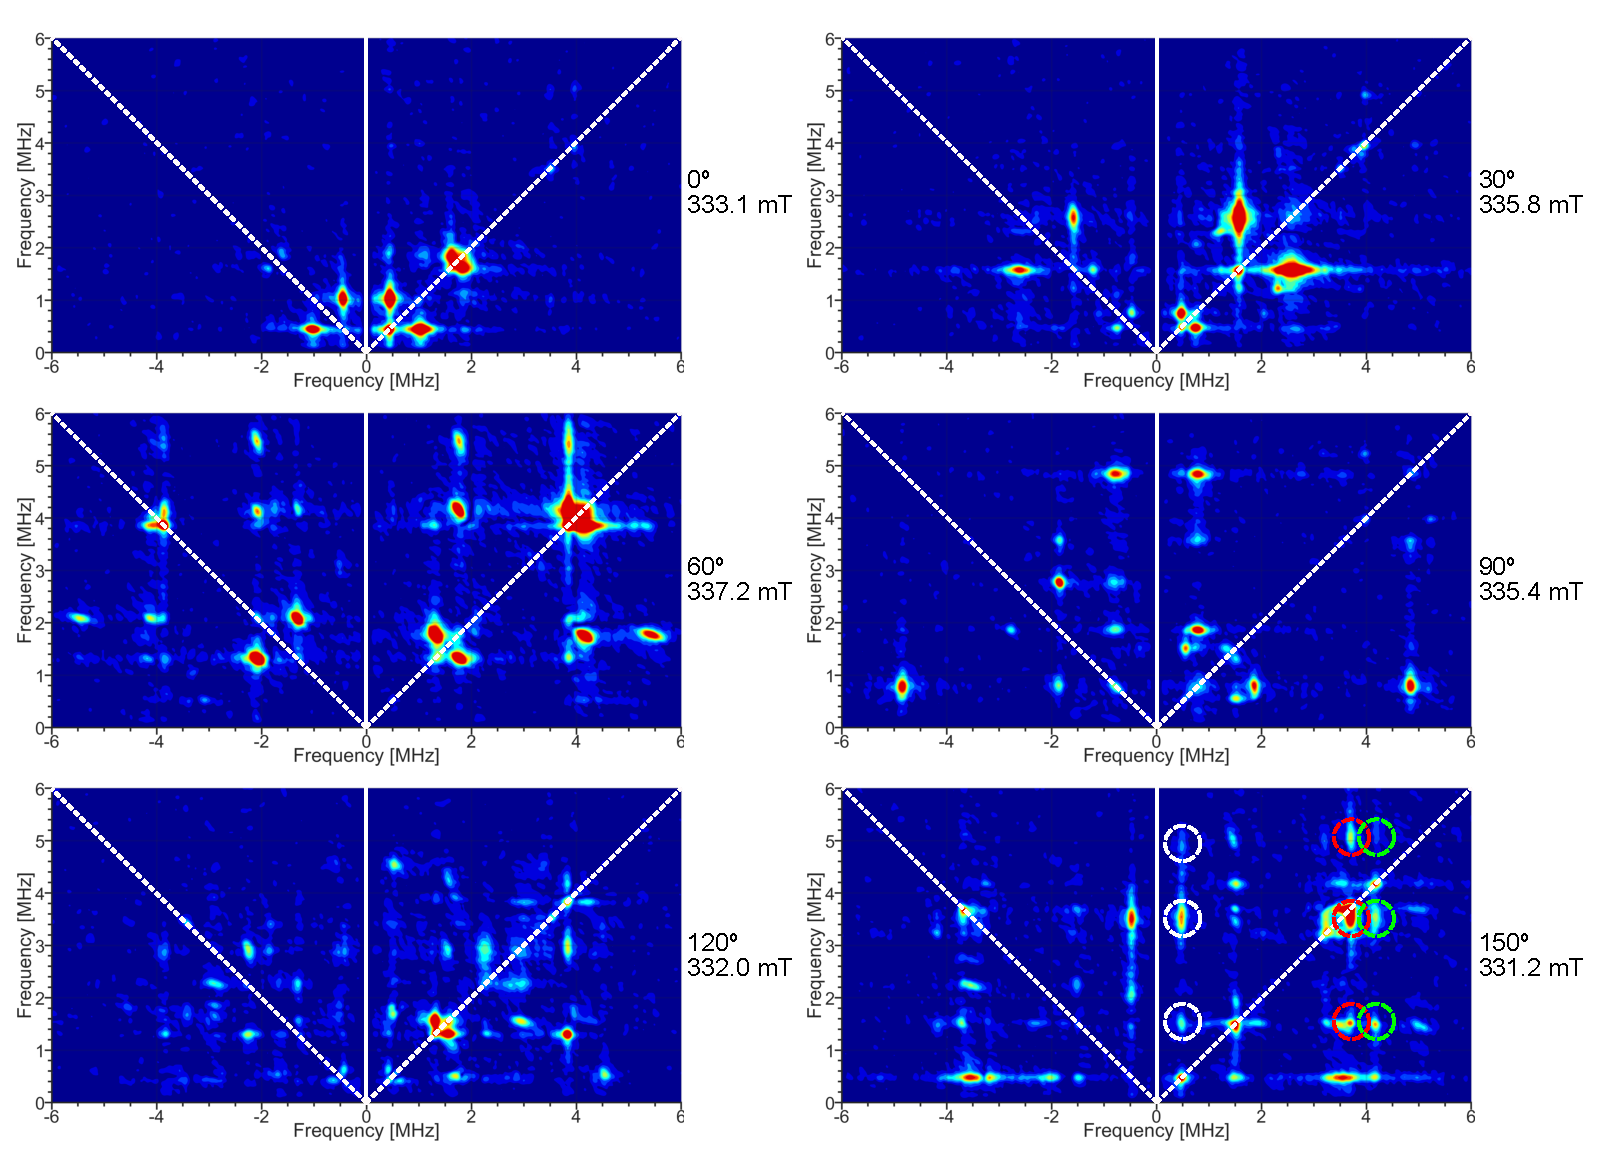
\includegraphics[width=\textwidth]{Kapitel/Ch5-Images/FeFe-FollowHyscore.eps}
 \caption[Single-crystal HYSCORE EPR following a single peak.]{Single-crystal HYSCORE EPR following the fuchsia-colored resonance roadmap of Fig.~\ref{fig:xTalFeFe}A.} \label{fig:FeFeHYSCOREFollow}
\end{figure}

In a HYSCORE experiment, the 2D density representation shows correlations between the nuclear-spin transitions (m$_\text{I}$) in both projections of the electron spin. Both, the $^{14}$N nucleus ($I=1$) from a distal cyanide-ligand (CN$_\text{d}^-$) and the secondary-amine group in the azapropane-dithiolate-ligand (ADT-ligand) can potentially contribute to the HYSCORE spectrum generating three transitions per ligand for each electron-spin transition (m$_\text{S}$) manifold for a maximum of 12 modulation frequencies. According to an earlier study on H$_{ox}$ in frozen solution, the features of the distal cyanide-ligand spread out up to 6 MHz, while the transitions of the ADT-amine nitrogen are found between 2 and 4~MHz. \cite{Adamska2015,Adamska2015pdt}

Currently, the full hyperfine- and quadrupole-tensor has not been solved. However, we can compare the data that was collected with previous work and gain further insight. For example, in Fig.~\ref{fig:FeFeHYSCOREFollow} at 0 and 30 degrees a strong signal can be seen in the weak coupling (++) quadrant under a coupling frequency of 4~MHz. These signals are attributed to the ADT-ligand and fit the principle values described in Adamska {\textit et al.} \cite{Adamska2015pdt} As the HYSCORE data is rotated these signals are reduced and signals with larger couplings are found in the 4 to 6~MHz range, including signals in the strong coupling ($-+$) quadrant. These signals are best represented by the distal cyanide-ligand (CN$_\text{d}^-$) as descrbed in a second paper by Adamska {\textit et al.} \cite{Adamska2015}.

A second data set of ESEEM was performed following the fuchsia-colored resonance roadmap of Appendix D Fig.~D.1 and plotted in Fig.~\ref{fig:ESEEM2}. These ESEEM data were performed at a finer resolution of 5 degree steps over 180 degree rotation. From this data we can 

\begin{figure}[ht]
\centering
 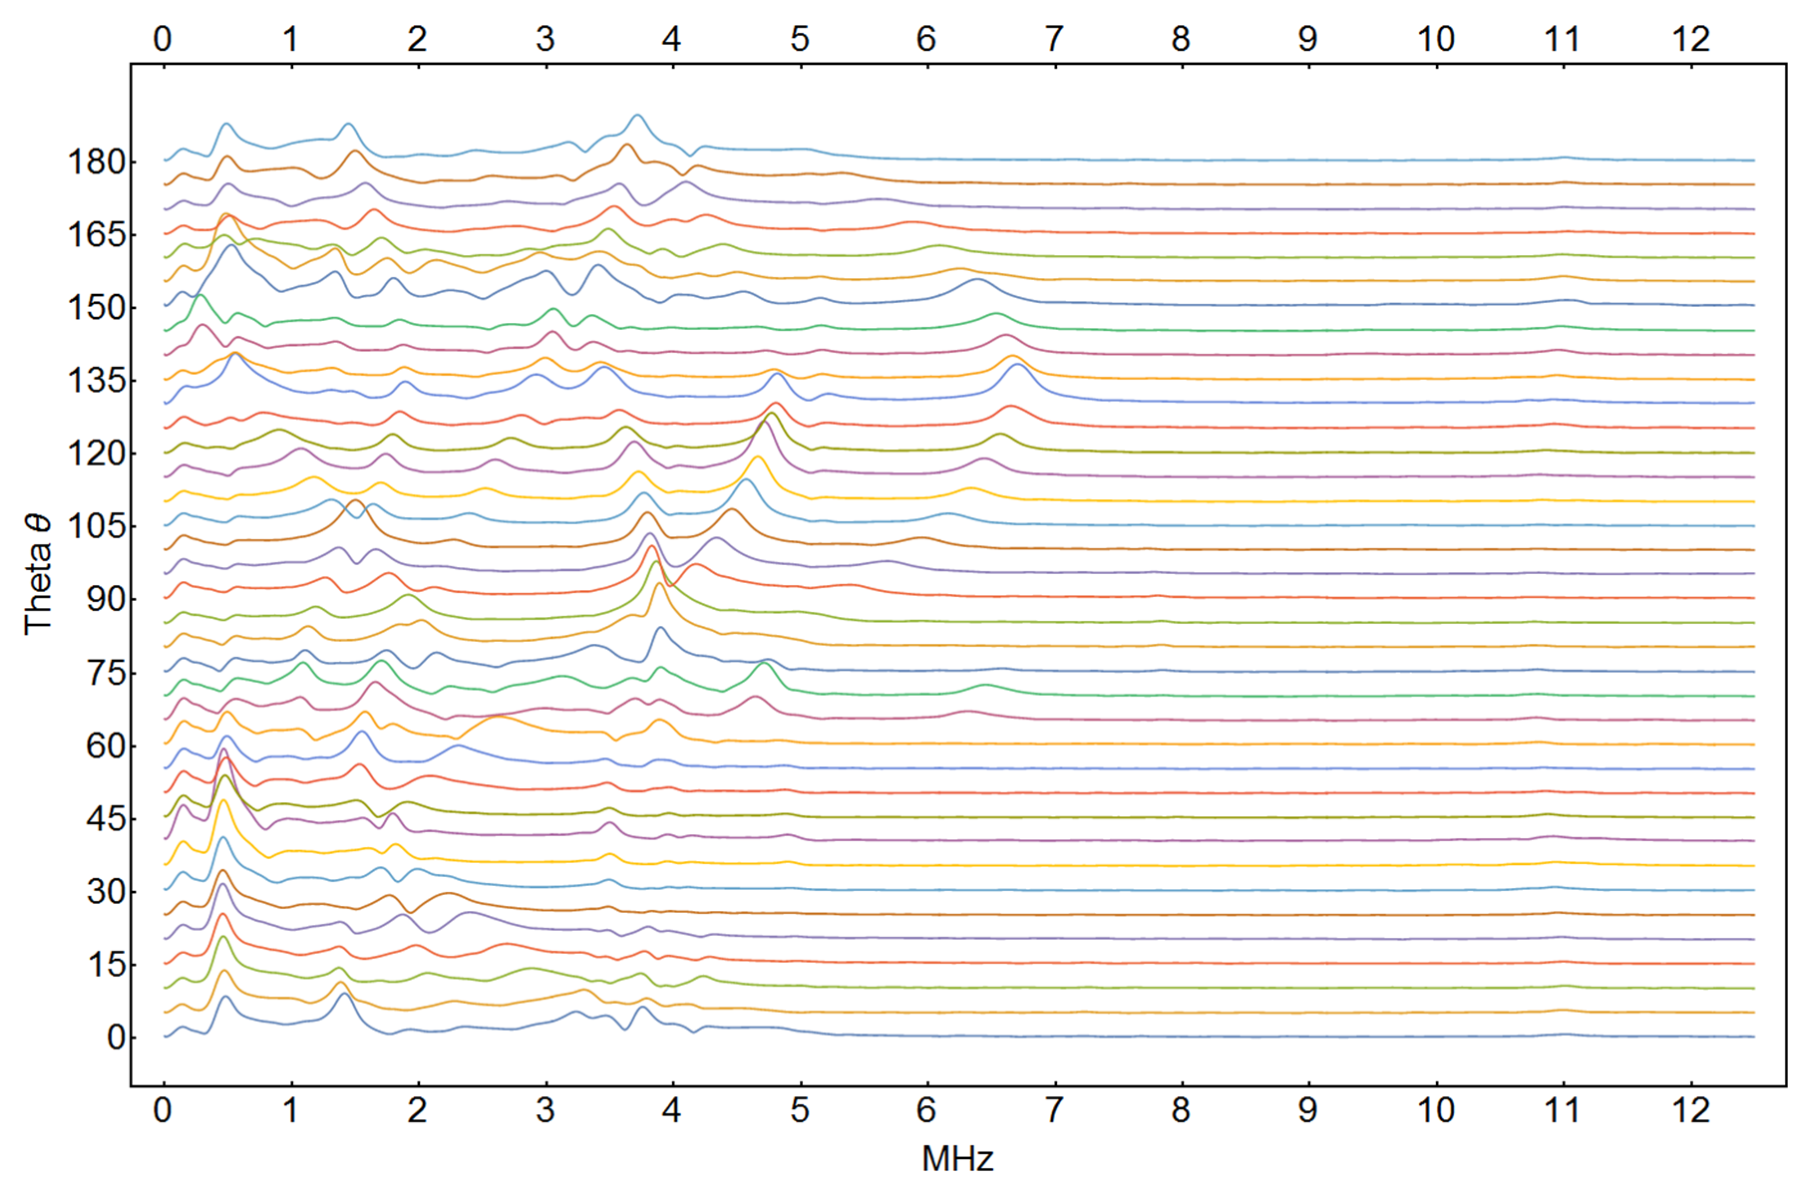
\includegraphics[width=0.8\textwidth]{Kapitel/Appendix/ESEEMFirstPeak.eps}
 \caption[Single-crystal ESEEM EPR: Fuchsia Trace.]{Single-crystal ESEEM EPR following the fuchsia-colored resonance roadmap of Fig.~D.1.} \label{fig:ESEEM2}
\end{figure}

\section{Conclusions and Outlook}
In this work we have demonstrated that a full angular $g$-tensor determination can be performed on crystals smaller than 27~nL volumes with excellent signal-to-noise at X-band. The proposed $g$-tensor is a refinement on previous work by Adamska {\em et al.}, which used orientation-selection HYSORE on frozen-solution samples at X-band and Q-band to back project the $g$-tensor. In this work, no assumptions are made and the $g$-tensor is measured directly. Although a single plane was rotated, the P$1\,2_1\,1$ symmetry of the crystal and the orientation of the crystal in the Laboratory Frame has allowed for a good fit. 

This work also demonstrates the ability to perform HYSCORE experiment on the same crystal and highlights the feasibility of such advanced EPR experiment. Future ESEEM/HYSCORE experiments will address the $^{14}$N couplings of the CN$^-$ and ADT ligands in greater detail. Possibly this will involve selective $^{15}$N labeling as has been demonstrated before. \cite{Adamska2015, AdamskaBridgingAmine} From such experiments, extracting the magnitude and orientation of the hyperfine- and nitrogen quadrupole-tensors in the molecular axis frame and relating these to the electronic structure as predicted through quantum chemical calculations are possible. 
\begin{figure*}[htbp]
\centering
 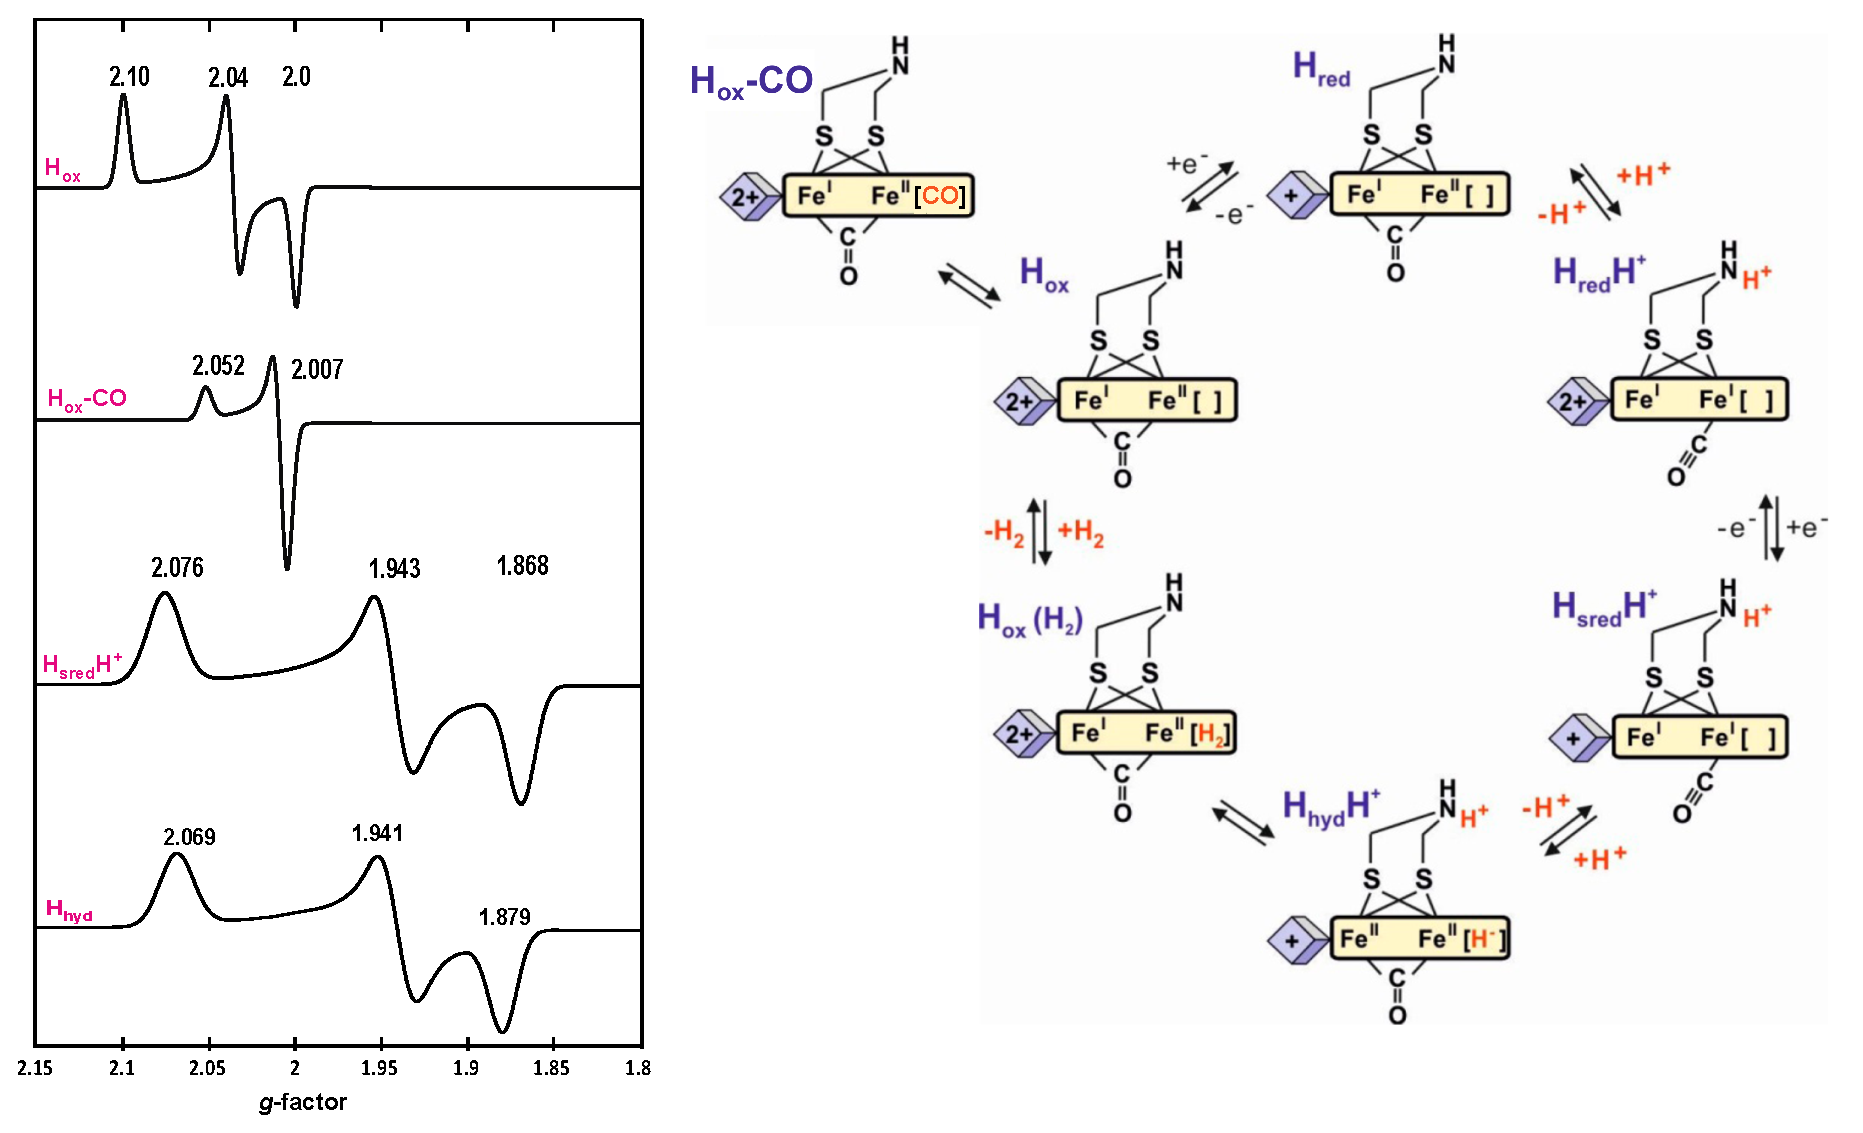
\includegraphics[width=\textwidth]{Kapitel/end-images/Ch6-EPRCat.eps}
 \caption[EPR Signals along the catalytic cycle of FeFe-Hydrogenase.]{Shown are simulations of the EPR signal from paramagnetic intermediates of frozen solution samples along the catalytic cycle of [FeFe]-hydrogenase is displayed on the left. A simplified catalytic cycle showing the redox states of the distal and proximal iron and [4Fe4S] clusters is displayed on the right.} 
 \label{fig:FeFeCatCycle}
\end{figure*}

Focusing on [FeFe]-hydrogenase, further studies of g-tensor and hyperfine-tensor interactions are now feasible in single-crystal experiments. Shown in Fig.~\ref{fig:FeFeCatCycle} are the simulations of the frozen solution spectra relating to the intermediates on the proposed catalytic cycle. \cite{lubitzhyd} Crystals of suitable size (0.8-3 nL) are available of the [FeFe]-hydrogenase CpI in the H$_{ox}$ state, studied herein, and a reduced CpI-apo which has an EPR signal derived from the reduced four [4Fe4S]$^+$ clusters. In CpI-apo, the H-cluster is not present. The CPI-apo crystal could be used to study the electron transfer pathway of the [FeFe]-hydrogenase and how it relates to the function of the hydrogenase at various redox potentials. It is also possible to obtain crystals in the inactive H$_{ox}$-CO state, which may lend insight into reducing the oxygen sensitivity of the [FeFe]-hydrogenase. Such studies will further protein engineering and artificial enzyme research for creating bio-inspired and bio-mimicking hydrogenase systems. \cite{C7SE00582B}


{\renewcommand{\bibsection}{\clearpage\section*{\bibname}\markboth{\bibname}{\bibname}}
\renewcommand{\bibname}{CHAPTER 6. REFERENCES}
\bibliographystyle{elsarticle-num}
\bibliography{Kapitel/Ch5-References}
}